\documentclass{article}

\usepackage{tikz}
\usepackage{tkz-graph}
\usepackage{tkz-berge}

\begin{document}
\begin{center}
  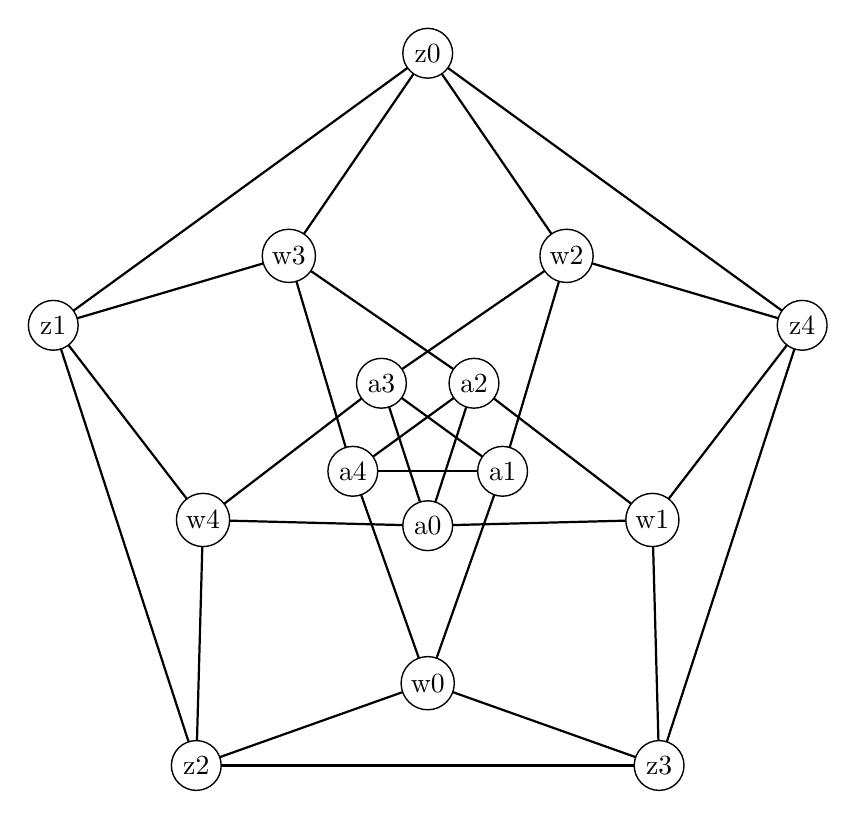
\begin{tikzpicture}
    \grEmptyCycle[RA=1,rotation=-90]{5}
    \grEmptyCycle[RA=3,prefix=w,rotation=-90]{5}
    \grCycle[RA=5,prefix=z,rotation=90]{5}
    \EdgeInGraphMod{a}{5}{2}
    \EdgeMod{a}{w}{5}{1}
    \EdgeMod{a}{w}{5}{-1}
    \EdgeMod{w}{z}{5}{2}
    \EdgeMod{w}{z}{5}{-2}    
  \end{tikzpicture}
\end{center}

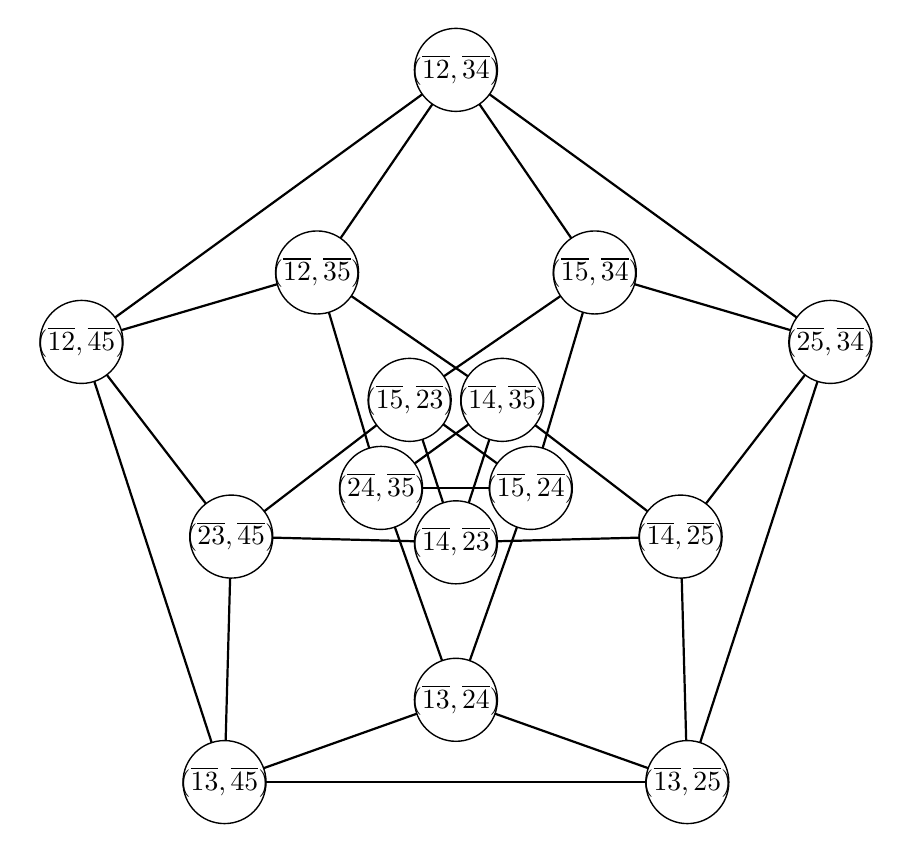
\begin{tikzpicture}%[rotate=90,scale=1]
  \newcommand{\aset}[2]{$\{#1,#2\}$}
  \GraphInit[vstyle=Classic]
  %\tikzset{VertexStyle/.style={draw,circle}}
  \SetVertexNoLabel
  \SetVertexMath
  \SetUpVertex[MinSize=30pt]
  \grEmptyCycle[RA=1,rotation=-90]{5}
  \grEmptyCycle[RA=3,prefix=w,rotation=-90]{5}
  \grCycle[RA=5,prefix=z,rotation=90]{5}
  \EdgeInGraphMod{a}{5}{2}
  \EdgeMod{a}{w}{5}{1}
  \EdgeMod{a}{w}{5}{-1}
  \EdgeMod{w}{z}{5}{2}
  \EdgeMod{w}{z}{5}{-2}   
  \AssignVertexLabel{z}{\textsl{$(\overline{12},\overline{34})$},\textsl{$(\overline{12},\overline{45})$},\textsl{$(\overline{13},\overline{45})$},\textsl{$(\overline{13},\overline{25})$},\textsl{$(\overline{25},\overline{34})$}}
  \AssignVertexLabel{w}{\textsl{$(\overline{13},\overline{24})$},\textsl{$(\overline{14},\overline{25})$},\textsl{$(\overline{15},\overline{34})$},\textsl{$(\overline{12},\overline{35})$},\textsl{$(\overline{23},\overline{45})$}}
  \AssignVertexLabel{a}{\textsl{$(\overline{14},\overline{23})$},\textsl{$(\overline{15},\overline{24})$},\textsl{$(\overline{14},\overline{35})$},\textsl{$(\overline{15},\overline{23})$},\textsl{$(\overline{24},\overline{35})$}}
\end{tikzpicture}

\begin{center}
  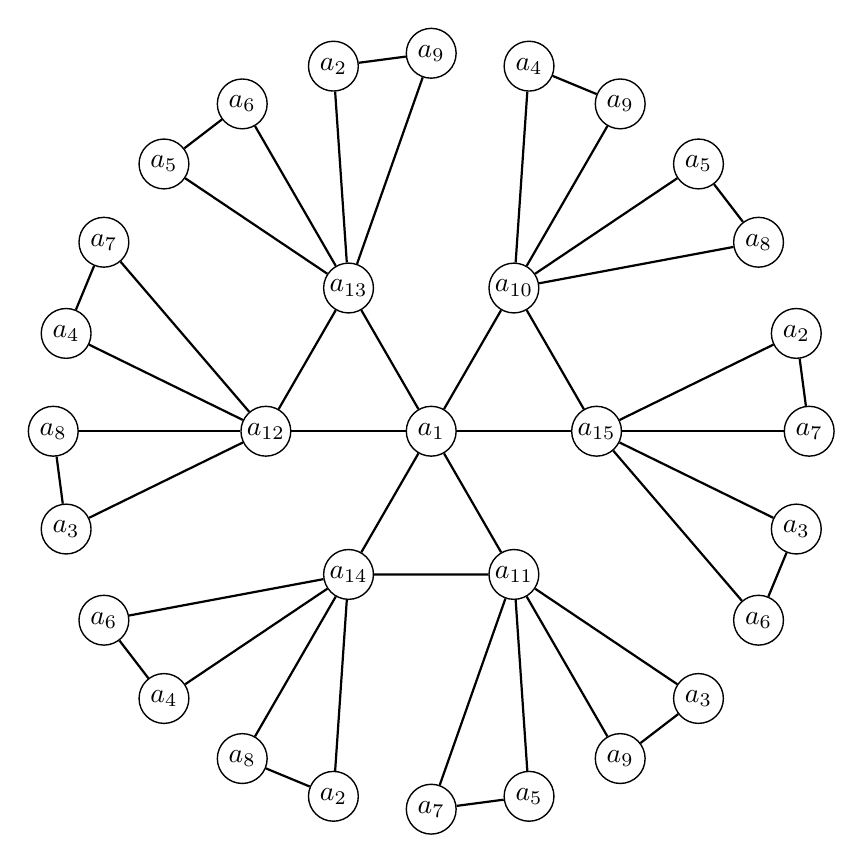
\begin{tikzpicture}[scale=.6]
    \GraphInit[vstyle=Normal] \SetVertexNoLabel
    \grStar[RA=3.5,Math]{7}%
    \grEmptyCycle[RA=8,prefix=c]{24} \EdgeInGraphMod*{a}{6}{1}{0}{2}
    \EdgeInGraphMod*{c}{24}{1}{0}{2} \EdgeFromOneToSeq{a}{c}{1}{2}{5}
    \EdgeFromOneToSeq{a}{c}{2}{6}{9}
    \EdgeFromOneToSeq{a}{c}{3}{10}{13}
    \EdgeFromOneToSeq{a}{c}{4}{14}{17}
    \EdgeFromOneToSeq{a}{c}{5}{18}{21}
    \EdgeFromOneToSeq{a}{c}{0}{22}{23}
    \EdgeFromOneToSeq{a}{c}{0}{0}{1}
    \AssignVertexLabel{a}{\textsl{$a_{15}$},\textsl{$a_{10}$},\textsl{$a_{13}$},\textsl{$a_{12}$},\textsl{$a_{14}$},\textsl{$a_{11}$},\textsl{$a_{1}$}}
    \AssignVertexLabel{c}{\textsl{$a_{7}$},\textsl{$a_{2}$},\textsl{$a_{8}$},\textsl{$a_{5}$},\textsl{$a_{9}$},\textsl{$a_{4}$},\textsl{$a_{9}$},\textsl{$a_{2}$},\textsl{$a_{6}$},\textsl{$a_{5}$},\textsl{$a_{7}$},\textsl{$a_{4}$},\textsl{$a_{8}$},\textsl{$a_{3}$},\textsl{$a_{6}$},\textsl{$a_{4}$},\textsl{$a_{8}$},\textsl{$a_{2}$},\textsl{$a_{7}$},\textsl{$a_{5}$},\textsl{$a_{9}$},\textsl{$a_{3}$},\textsl{$a_{6}$},\textsl{$a_{3}$}}
  \end{tikzpicture}
\end{center}

\begin{figure}[h]
  \centering
  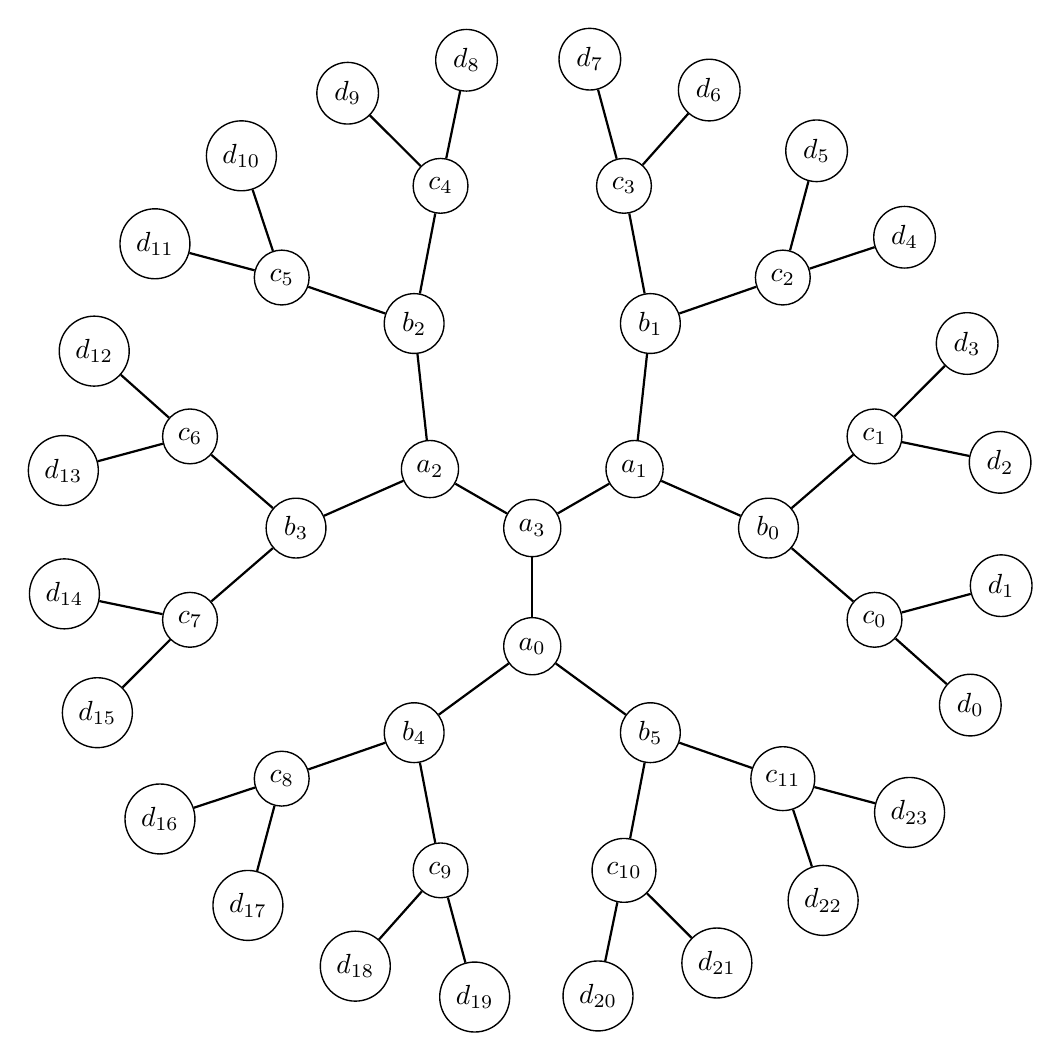
\begin{tikzpicture}[scale=.5]
    \GraphInit[vstyle=Normal] %\SetVertexNoLabel
    \grStar[RA=3,Math,rotation=270]{4}
    \grEmptyCycle[RA=6,Math,prefix=b]{6} 
    \grEmptyCycle[RA=9,Math,prefix=c,rotation=-15]{12} 
    \grEmptyCycle[RA=12,Math,prefix=d,rotation=-22]{24} 
    \EdgeFromOneToSeq{a}{b}{1}{0}{1}
    \EdgeFromOneToSeq{a}{b}{2}{2}{3}
    \EdgeFromOneToSeq{a}{b}{0}{4}{5}
    \EdgeFromOneToSeq{b}{c}{0}{0}{1}
    \EdgeFromOneToSeq{b}{c}{1}{2}{3}
    \EdgeFromOneToSeq{b}{c}{2}{4}{5}
    \EdgeFromOneToSeq{b}{c}{3}{6}{7}
    \EdgeFromOneToSeq{b}{c}{4}{8}{9}
    \EdgeFromOneToSeq{b}{c}{5}{10}{11}
    \EdgeFromOneToSeq{c}{d}{0}{0}{1}
    \EdgeFromOneToSeq{c}{d}{1}{2}{3}
    \EdgeFromOneToSeq{c}{d}{2}{4}{5}
    \EdgeFromOneToSeq{c}{d}{3}{6}{7}
    \EdgeFromOneToSeq{c}{d}{4}{8}{9}
    \EdgeFromOneToSeq{c}{d}{5}{10}{11}
    \EdgeFromOneToSeq{c}{d}{6}{12}{13}
    \EdgeFromOneToSeq{c}{d}{7}{14}{15}
    \EdgeFromOneToSeq{c}{d}{8}{16}{17}
    \EdgeFromOneToSeq{c}{d}{9}{18}{19}
    \EdgeFromOneToSeq{c}{d}{10}{20}{21}
    \EdgeFromOneToSeq{c}{d}{11}{22}{23}
  \end{tikzpicture}
  
  \caption{Gráfica de .....}
  \label{fig:emparejamiento6}
\end{figure}

%\begin{center}
 % \begin{tikzpicture}
  %  \grEmptyCycle[RA=2,prefix=v,rotation=180,Math]{3} 
   %  \Edge[style={->}](v0)(v1)
    %\Edge(v1)(v2)
    %\Edge(a)(b)
  %\end{tikzpicture}
%\end{center}

\begin{center}
     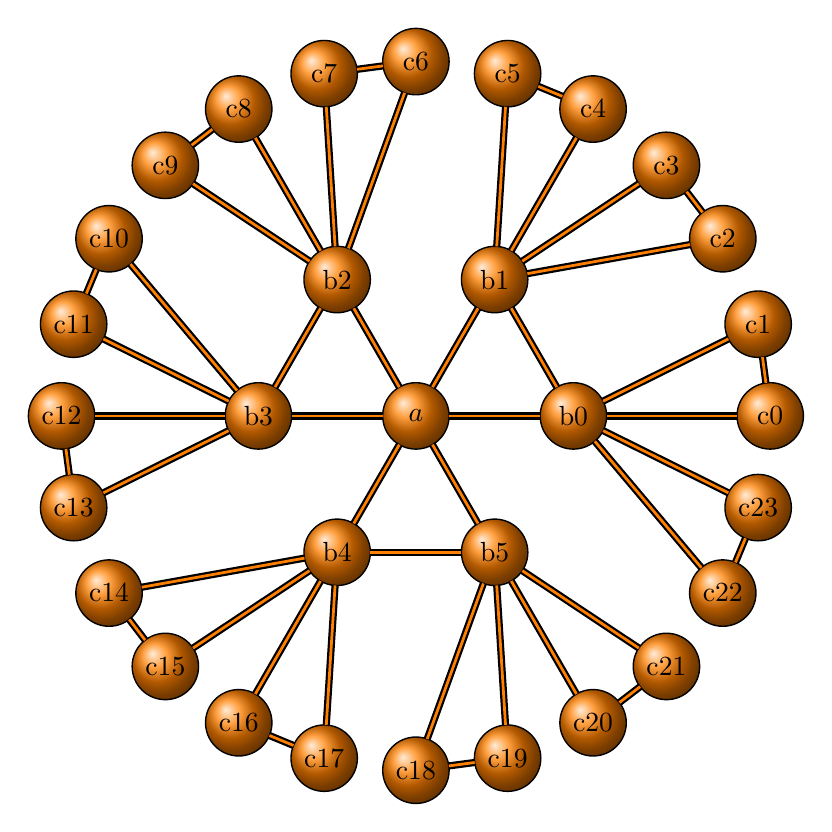
\begin{tikzpicture}
       \GraphInit[vstyle=Shade]
       \Vertex[x=0,y=0,Math]{a}
       \grEmptyCycle[RA=2,prefix=b]{6}
       \grEmptyCycle[RA=4.5,prefix=c]{24}
       \EdgeFromOneToAll{a}{b}{}{6}
       \EdgeInGraphMod*{b}{6}{1}{0}{2}
       \EdgeInGraphMod*{c}{24}{1}{0}{2}
       \EdgeFromOneToSeq{b}{c}{1}{2}{5}
       \EdgeFromOneToSeq{b}{c}{2}{6}{9}
       \EdgeFromOneToSeq{b}{c}{3}{10}{13}
       \EdgeFromOneToSeq{b}{c}{4}{14}{17}
       \EdgeFromOneToSeq{b}{c}{5}{18}{21}
       \EdgeFromOneToSeq{b}{c}{0}{22}{23}
       \EdgeFromOneToSeq{b}{c}{0}{0}{1}
     \end{tikzpicture}
\end{center}

\begin{center}
  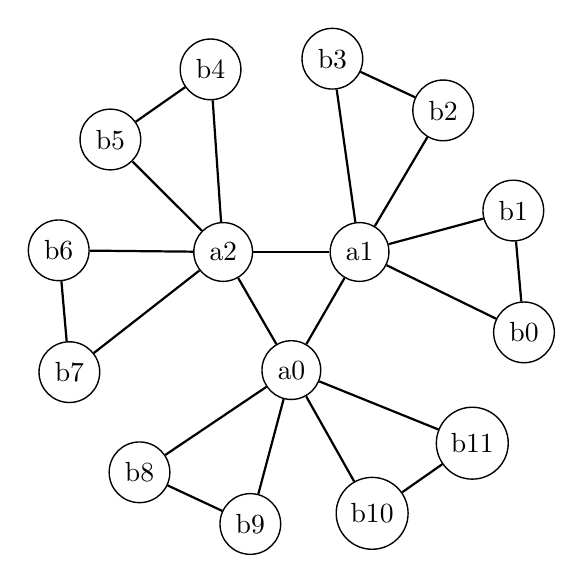
\begin{tikzpicture}
    \GraphInit[vstyle=Normal]
    %\SetVertexNoLabel
    \grCycle[RA=1,prefix=a,rotation=-90]{3}
    \grEmptyCycle[RA=3,prefix=b,rotation=-10]{12}
    \EdgeInGraphMod*{b}{12}{1}{0}{2}
    \EdgeFromOneToSeq{a}{b}{1}{0}{3}
    \EdgeFromOneToSeq{a}{b}{2}{4}{7}
    \EdgeFromOneToSeq{a}{b}{0}{8}{11}
  \end{tikzpicture}
\end{center}

\begin{center}
  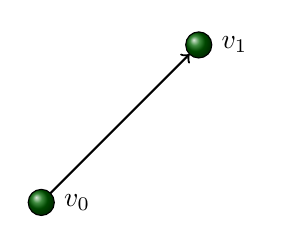
\begin{tikzpicture}
    \GraphInit[vstyle=Classic]
    \tikzset{VertexStyle/.style = {%
        shape= circle,
        shading= ball,
        ball color= green!40!black,%
        minimum size = 2pt,draw}}
    \Vertex[x=0,y=0,Math]{v_{0}}
    \Vertex[x=2,y=2,Math]{v_{1}}
    \Edge[style={->}](v_{0})(v_{1})
  \end{tikzpicture}
\end{center}

\begin{center}
  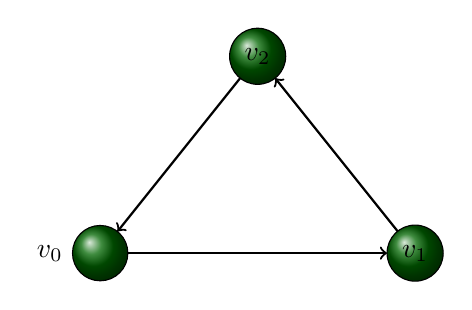
\begin{tikzpicture}
    \draw[help lines] (-2,0);% grid (2,3);
    %\SetGraphUnit{2}
    \GraphInit[vstyle=Normal]
    \SetUpVertex[MinSize=0.5pt]
    \tikzset{VertexStyle/.style = {%
        shape= circle,
        shading= ball,
        ball color= green!40!black,%
        minimum size = 20pt,draw}}
    \Vertex[x=-2,y=0,Math,LabelOut,Lpos=180,]{v_{0}}
    \Vertex[x=2,y=0,Math]{v_{1}}
    \Vertex[x=0,y=2.5,Math]{v_{2}}
    \Edge[style={->}](v_{0})(v_{1})
    \Edge[style={->}](v_{1})(v_{2})
    \Edge[style={->}](v_{2})(v_{0})
 \end{tikzpicture}
\end{center}

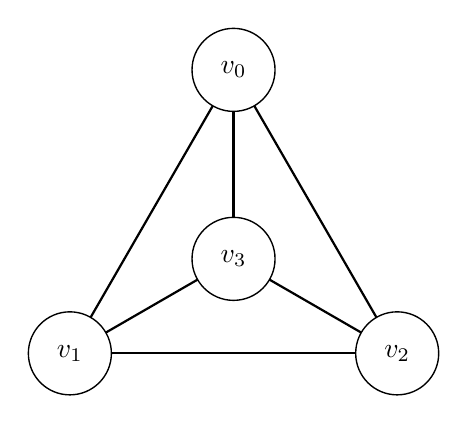
\begin{tikzpicture}[scale=.6]
  \GraphInit[vstyle=Classic]
  \SetVertexNoLabel
  \SetVertexMath
  \SetUpVertex[MinSize=30pt]
  \grTetrahedral[RA=4]
  \AssignVertexLabel{a}{\textsl{$v_{0}$},\textsl{$v_{1}$},\textsl{$v_{2}$},\textsl{$v_{3}$}}
\end{tikzpicture}

\end{document}
